\chapter{Limitations of Affine Normalizing Flows}\label{ch:04}

\begin{remark}{Outline}
  Here, we draw connections between normalizing flows and Bayesian networks. These guide our proofs of three essential properties of affine normalizing flows.
  First, we show that stacking multiple transformations in a normalizing flow relaxes independence assumptions and entangles the model distribution.
  Second, we show that a fundamental leap of capacity emerges when the depth of affine flows exceeds three transformation layers.
  Third, we prove the non-universality of the affine normalizing flow, regardless of its depth.
\end{remark}

\section{Prologue}
This chapter highlights the relevance of bridging distinct classes of probabilistic models together. These connections provide new viewpoints that can help us focus on some models' components and abstract others less relevant to what we want to understand.

In this specific case, we derive properties of affine normalizing flows that have significant consequences for the practitioners who want to use normalizing flows. In many cases, the best choice is to stack three steps of normalizing flows. Not more. Adding more will unnecessarily slow down the inversion of the flow. On the contrary, increasing the capacity of each step will only marginally impact the sampling complexity. Provably, the latter solution is as expressive as the former but has a reduced cost.

This chapter shall convince the reader that gaining theoretical understanding of probablistic models is key for using these models appropriately. To this purpose, taking a new perspective by drawing connections between different types of models, here graphical and deep probablistic models, is an efficient solution. With simple analogies we are then able to reason intuitivly on the class of models.

Without further ado, we invite the reader to overview the next section and jump into the publication.
\section{The paper: You say Normalizing Flows I see Bayesian Networks}

\subsection{Author contributions}
The paper is co-authored by me and Gilles Louppe. As the leading author, I developed the connections between normalizing flows and Bayesian networks, made the experiments, and wrote the paper. Gilles Louppe supervised me throughout this project, offered suggestions and helped in writing the paper.

\subsection{Reading tips}
The reader may skip section 2 which presents normalizing flows and Bayesian networks already introduced the background chapter. We also encourage the reader to first focus on understanding the relationship between Figure~1 and coupling layers presented in section~3.2. The reader can then focus on understanding section~3.3 which provides the ground for the rest of the paper.
% \subsection{Minor corrections}
\includepdf[pages=-]{papers/innf.pdf}

\section{Epilogue}
\subsection{Scientific impact}
\begin{figure}
  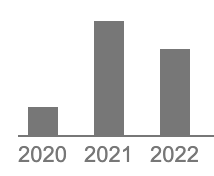
\includegraphics[width=.2\textwidth]{figures/impact_scholar/You_say_I_see.png}
  \caption{}
  \label{}
\end{figure}

After the publication of this short article, the idea of combining NFs and BNs has led to Graphical Normalizing Flows, which are later presented in \Cref{ch:06}. At the same workshop, \citet{khemakhem_causal_2020} presented connections between autoregressive NFs and causal networks, sub-class of BNs featured with causal interpretation. Subsequent work has also focused on combining probabilistic graphical models with normalizing flows such as \citet{mouton2022graphical, mouton2022siren}.

We regret that our work has not gained more attention from practitioners who use affine normalizing flows. Indeed, it is still widespread to encounter publications that stack tens of NF steps (e.g., \citep{daxamortized}). This still happens, although other work reached the same conclusion regarding the number of steps in affine NFs. In particular, \citet{koehler2021representational} shows that three steps of affine coupling flows are sufficient to express any distribution on $\mathbb{R}^d$. On the one hand, this result aligns with ours, which says stacking more than three steps does not increase the expressivity of an NF.
On the other hand, it also contradicts our statement about the non-universality of affine flows. We explain this by observing that \citet{koehler2021representational} allows degenerate flows, flows for which the Jacobian explodes or shrinks, which corresponds to non-invertibility and is discarded in our discussion. Indeed, \citet{behrmann2021understanding} also shows that exploding Jacobians can cause numerical instabilities with the training and sampling of NFs.

\subsection{Conclusion and opportunities}
It is now clear that stacking more than three steps does not increase the expressivity of the class of models. However, it is unclear whether the training of flows gets simpler or more demanding by stacking steps, potentially more than three. Indeed the log-likelihood of a flow directly uses the Jacobian of each step; this may act as some skip connection in the gradient flow and potentially overcome potential gradient explosion or vanishing in deep neural networks with no skip connections. In the following chapter, we do not address this question; however, we introduce a new transformation that can significantly improve the expressivity of each normalizing flow step. This transformation allows us to reduce further the number of steps required and even achieves universal density approximation.
